\section{Introduction}
Microservice resource forecasts can provide inputs to capacity planning and autoscaling, but a forecast of recorded CPU or memory usage does not directly estimate unconstrained demand or demonstrate a better controller. Telemetry can be unavailable when collectors, transport or services fail. A forecaster must then separate the last observed value from the availability of that value, and its computational cost must remain appropriate for the monitoring setting. Work on workload learning, decomposition-based autoscaling and resource forecasting provides the application context \cite{powerprediction,autoscaling2025,temposcale,aero}. The present study evaluates point forecasts; it does not implement a controller or measure energy, service-level violations or cloud bills.

A second motivation concerns the interpretation of temporal decomposition. DLinear combines affine predictions from a fixed moving-average trend and its residual \cite{dlinear}. With a fixed linear smoothing operator, their sum is an affine function of the input window. Reducing the parameterization therefore need not introduce a new function class. Availability-dependent smoothing and explicit missingness descriptors are different interventions, and empirical gains cannot be inferred from either algebraic equivalence or a smaller parameter count. This distinction is particularly relevant when a small model is presented as an architectural improvement.

This work extends an existing, already inspected experiment on 28 ChronoGraph services. All historical artifacts remain separate from new evidence. We evaluate source-trained models on 32 additional services, with prefix-only destination calibration, and on a short external Alibaba 2022 case. The source and additional services share an infrastructure and observation period. Consequently, the primary evaluation is a predeclared spatial-transfer experiment, not an independently blinded temporal replication. An immutable local protocol and checkpoint freezes precede the corresponding target evaluations; they are not a public preregistration.

The contribution is an auditable empirical study rather than a claim of a universally superior architecture. It comprises (i) a compact affine parameterization with two separately ablated availability descriptors; (ii) paired evaluation of 15 families under ten missingness conditions, with ten seeded neural fits in the primary setting; (iii) direct-horizon and history-length extensions, plus calibrated external transfer; and (iv) independently reconstructed saved-prediction metrics and measured CPU/CUDA inference costs. Negative outcomes and limitations are retained.

\subsection{Research questions and evidence boundaries}
The research questions are: RQ1, how do error levels change with incomplete telemetry? RQ2, how do fixed decomposition, availability-dependent smoothing and compact parameterizations trade accuracy against cost? RQ3, when are missing-fraction and age descriptors useful? RQ4, does a compact affine model retain accuracy with fewer parameters? RQ5, how do conclusions change across services, direct horizons and datasets? RQ6, how much variation occurs across seeded fits, masks and time periods?

The operational primary hypothesis compares A3 with DLinear and E5 separately for CPU and memory. Four two-sided contrasts were specified; no improvement is required for completion. Missingness monotonicity, descriptor ablations, added stress mechanisms, horizon/history effects and external transfer are descriptive secondary analyses. The historical experiment motivated these hypotheses and remains exploratory. Fig.~\ref{fig:flow} summarizes the separation of evidence.
\begin{figure*}[!t]\centering
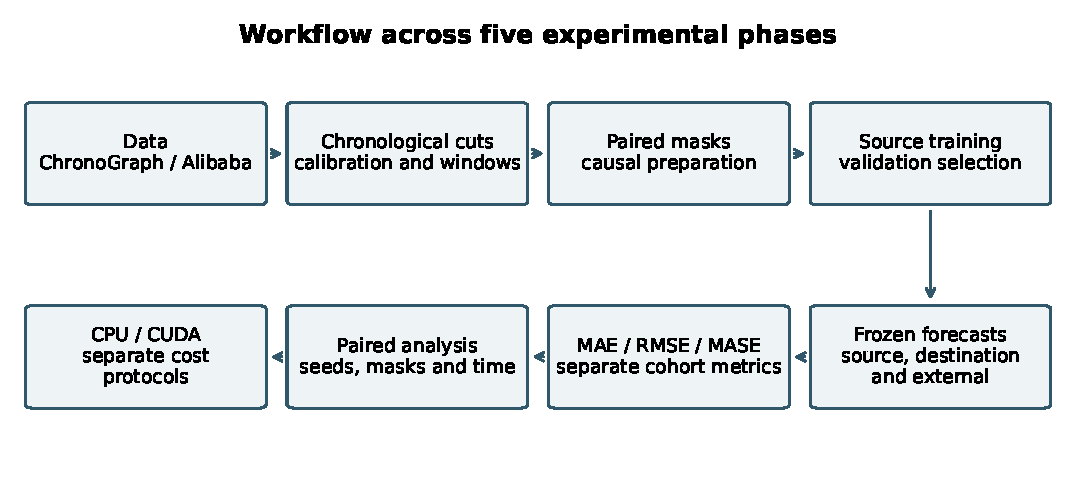
\includegraphics[width=0.93\textwidth]{figuras/01_methodology.pdf}
\caption{Study flow. Model selection and weights use only the 28-service source training/validation periods. The 32 destination services supply their training-prefix calibration statistics, not destination fitting or hyperparameter selection. Alibaba uses a separate six-hour calibration prefix.}\label{fig:flow}
\end{figure*}
